\documentclass{beamer}
\usepackage{amssymb, amsfonts, latexsym, amsthm, amsmath, framed, esvect, parskip}
\usepackage{amsmath, amssymb, framed, tcolorbox, mathrsfs, xcolor, graphicx}
\usepackage{multirow,booktabs, makecell}
\usepackage[backend=biber,style=numeric,sorting=none]{biblatex}
\setbeamerfont{footnote}{size=\tiny}
\addbibresource{ref.bib}
\tcbuselibrary{theorems}
\usepackage{listings}
\definecolor{green}{rgb}{0,0.6,0}
\definecolor{gray}{rgb}{0.5,0.5,0.5}
\definecolor{mauve}{rgb}{0.58,0,0.82}
\lstset{
    frame=none,
    language=Java,
    showstringspaces=false,
    columns=fullflexible,
    basicstyle = \ttfamily\small,
    numbers=none,
    numberstyle=\tiny\color{gray},
    keywordstyle=\color{blue},
    commentstyle=\color{green},
    stringstyle=\color{mauve},
    breaklines=true,
    morekeywords={function},
    breakatwhitespace=true,
    tabsize=4
}

% Beamer theme setting
\definecolor{myteal}{cmyk}{0.5,0,0.15,0}
\usecolortheme[named=myteal]{structure}
\definecolor{my-yellow}{cmyk}{0,0.2,0.7,0,1.00}
\definecolor{my-blue}{cmyk}{0.80, 0.13, 0.14, 0.04, 1.00}
\definecolor{my-green}{cmyk}{0.4,0,0.4,0,1.00}
\tcbset{
defstyle/.style={fonttitle=\bfseries\upshape, colback=my-yellow!5,colframe=my-yellow!80!black},
theostyle/.style={fonttitle=\bfseries\upshape, colback=my-blue!5,colframe=my-blue!80!black},
corstyle/.style={fonttitle=\bfseries\upshape, colback=my-green!5,colframe=my-green!80!black},
}
\usetheme{Madrid}
\setbeamertemplate{itemize items}[triangle]
\setbeamertemplate{enumerate items}[default]

\title{Week 6 Report}
\author{Ben Chen}
\institute{Dept of Computer Science and Engineering, SUSTech}
\date{\today}

\begin{document}
\frame{\titlepage}

\begin{frame}{TOC}
\begin{table}[ht]
    \tiny
	\centering
	\begin{tabular}[c]{ccccc}
		\toprule
        Title & Conference & Institute & Authors & Idea \\
		\midrule
        \makecell{A Genetic Algorithm for \\ a Spectre Attack Agnostic \\ to Branch Predictors} & CARRV '23 & Telecom Paris & \makecell{Dorian Bourgeoisat \\ Laurent Sauvage}  & \makecell{Branch predictor independent \\ spectre attack.} \\ \\ 
        \makecell{BUSted!!! Microarchitectural \\ Side-Channel Attacks on \\ the MCU Bus Interconnect} & Oakland '24 & UMinho & \makecell{Cristiano Rodrigues \\ Daniel Oliveira \\ Sandro Pinto}  & \makecell{Contention on bus \\ between MCU and DMA. \\ Similar to interrupt} \\
		\bottomrule
	\end{tabular}
\end{table}
\end{frame}

\begin{frame}[fragile]{Genetic Algorithm for Spectre\cite{bourgeoisat-2023}}
\begin{lstlisting}
void gadget(int x) {
    if (x < array1_size)
        y = array2[array1[x] * CACHE_LINE_SIZE];
}
...
// attack
for (int i = 0; i < N_TRAIN; i++)
    gadget(0);
gadget(&secret - array1); // not working
\end{lstlisting}

Reason: BP changed from Gshare $\to$ TAGE-\textbf{L}.

Loop predictor kicks in, so no misprediction.
\end{frame}

\begin{frame}[fragile]{Genetic Algorithm for Spectre\cite{bourgeoisat-2023}}
Different implementations of branch predictors in RISC-V: needs a generic attack.

Intuition: \textbf{Evolutionary Algorithm} to find the training sequence.

\begin{table}
\begin{center}
\begin{tabular}[c]{|l|c|c|c|c|c|c|}
\hline
\textbf{Parameters} & \textbf{x[0]} & \textbf{x[1]} & \textbf{x[2]} & \textbf{x[3]} & \textbf{x[4]} & \textbf{...} \\
\hline
\textbf{Value} & 0 & 4 & 3 & 1 & ATTACK & \textbf{...} \\
\hline
\end{tabular}
\end{center}
\end{table}

using the code

\begin{lstlisting}
for (int i = 0; i < N_TRAIN; i++)
    gadget(x[i]);
\end{lstlisting}

\end{frame}

\begin{frame}{BUSted\cite{BUSted}}
\begin{figure}
    \begin{center}
        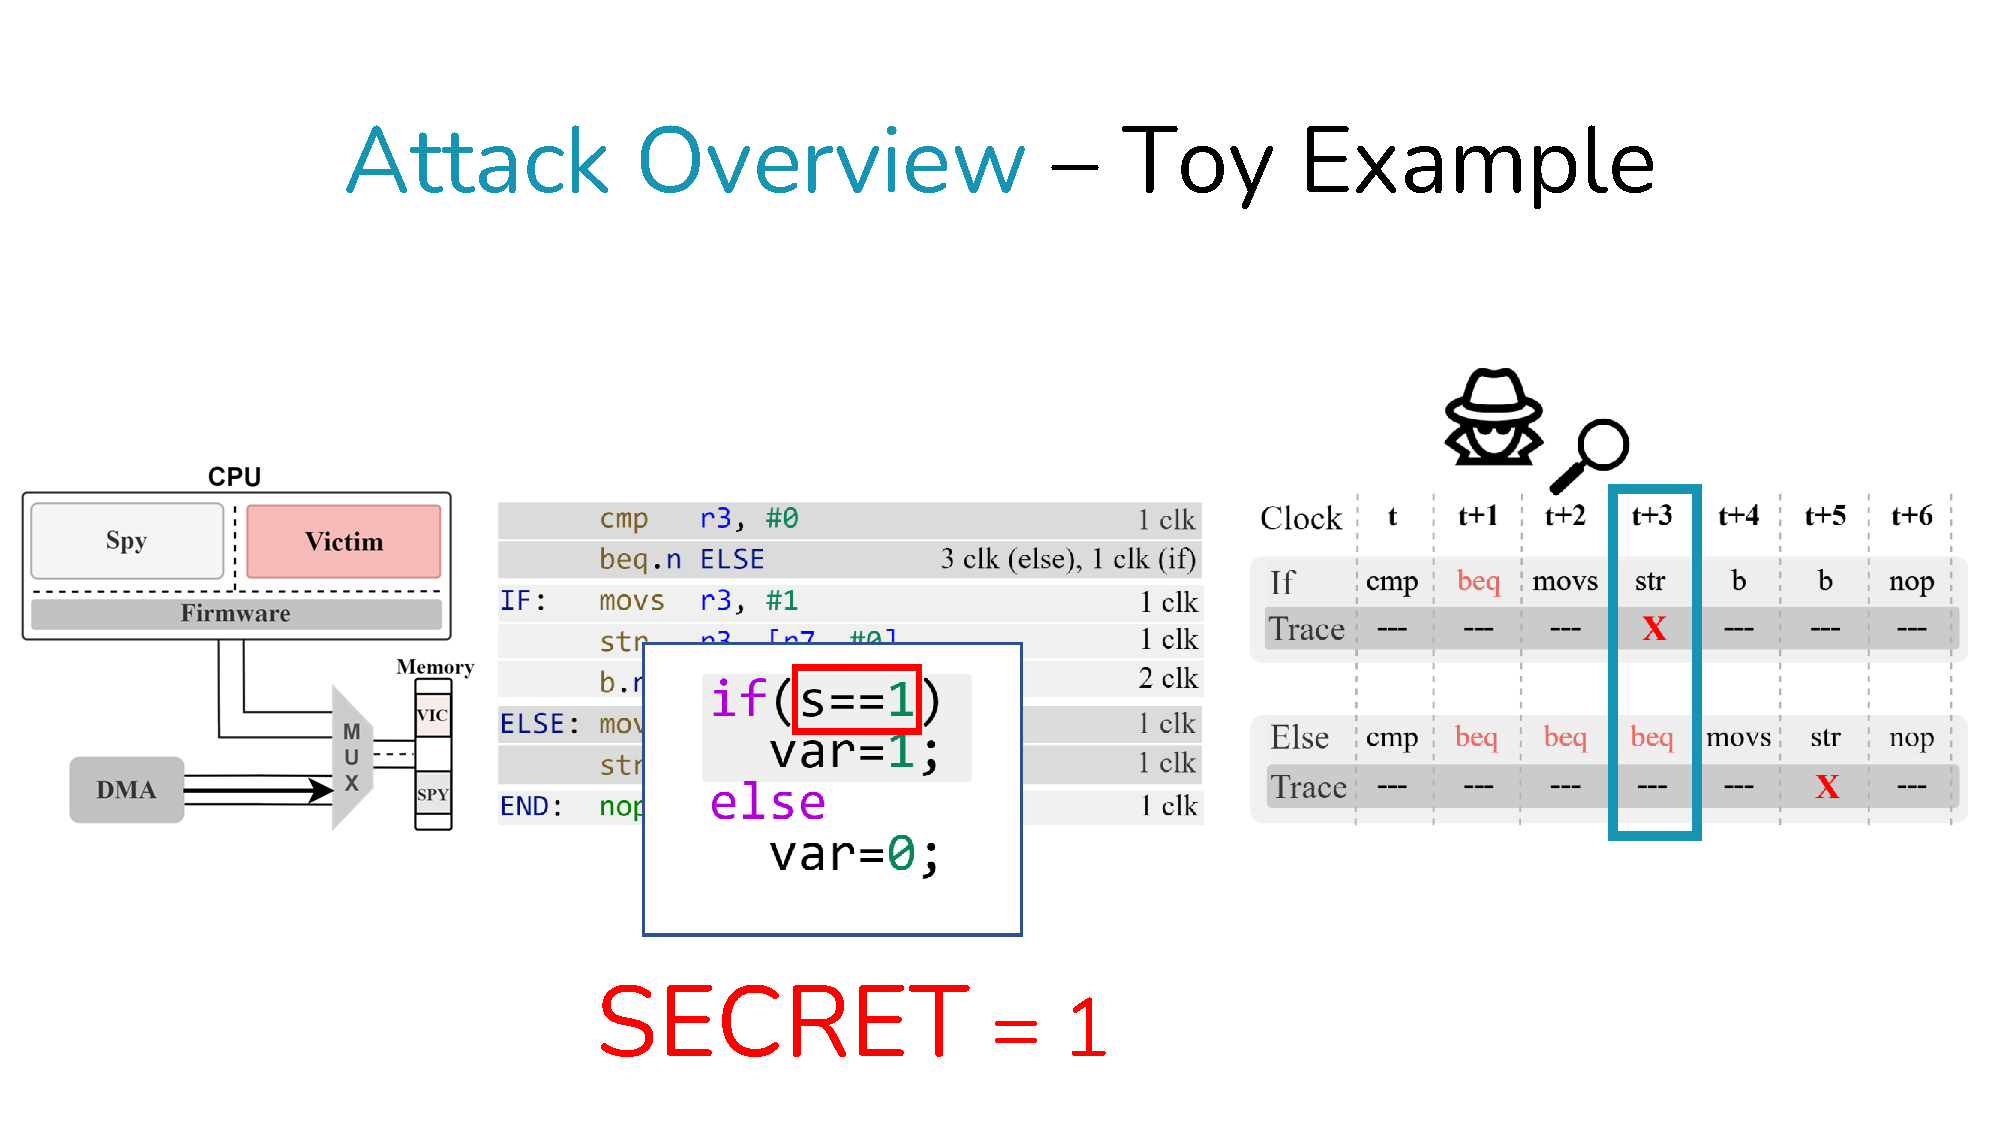
\includegraphics[width=1\textwidth]{img/busted1.pdf}
    \end{center}
\end{figure} 
\end{frame}

\begin{frame}{BUSted\cite{BUSted}}
\begin{figure}
    \begin{center}
        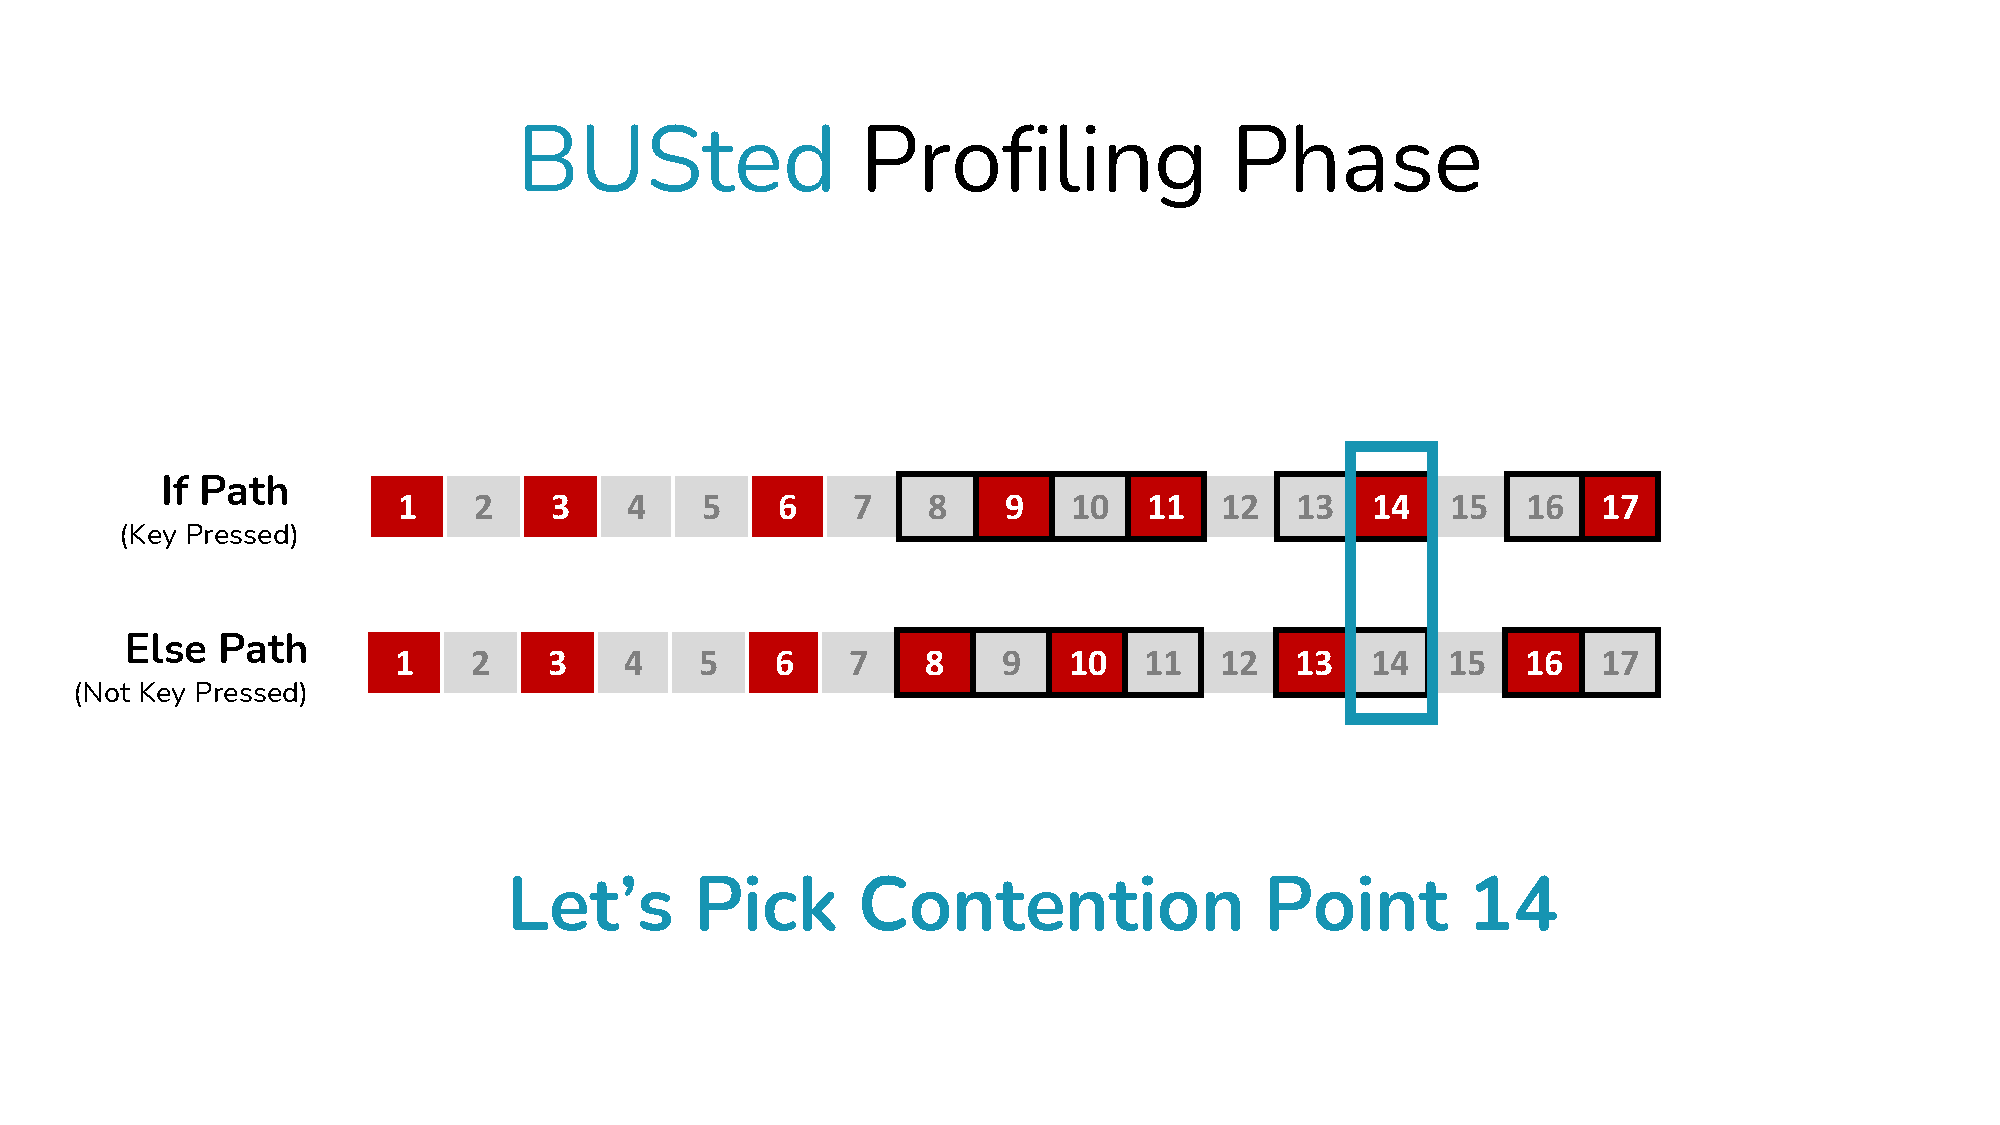
\includegraphics[width=1\textwidth]{img/busted2.pdf}
    \end{center}
\end{figure} 
\end{frame}

\begin{frame}{BUSted\cite{BUSted}}
\begin{figure}
    \begin{center}
        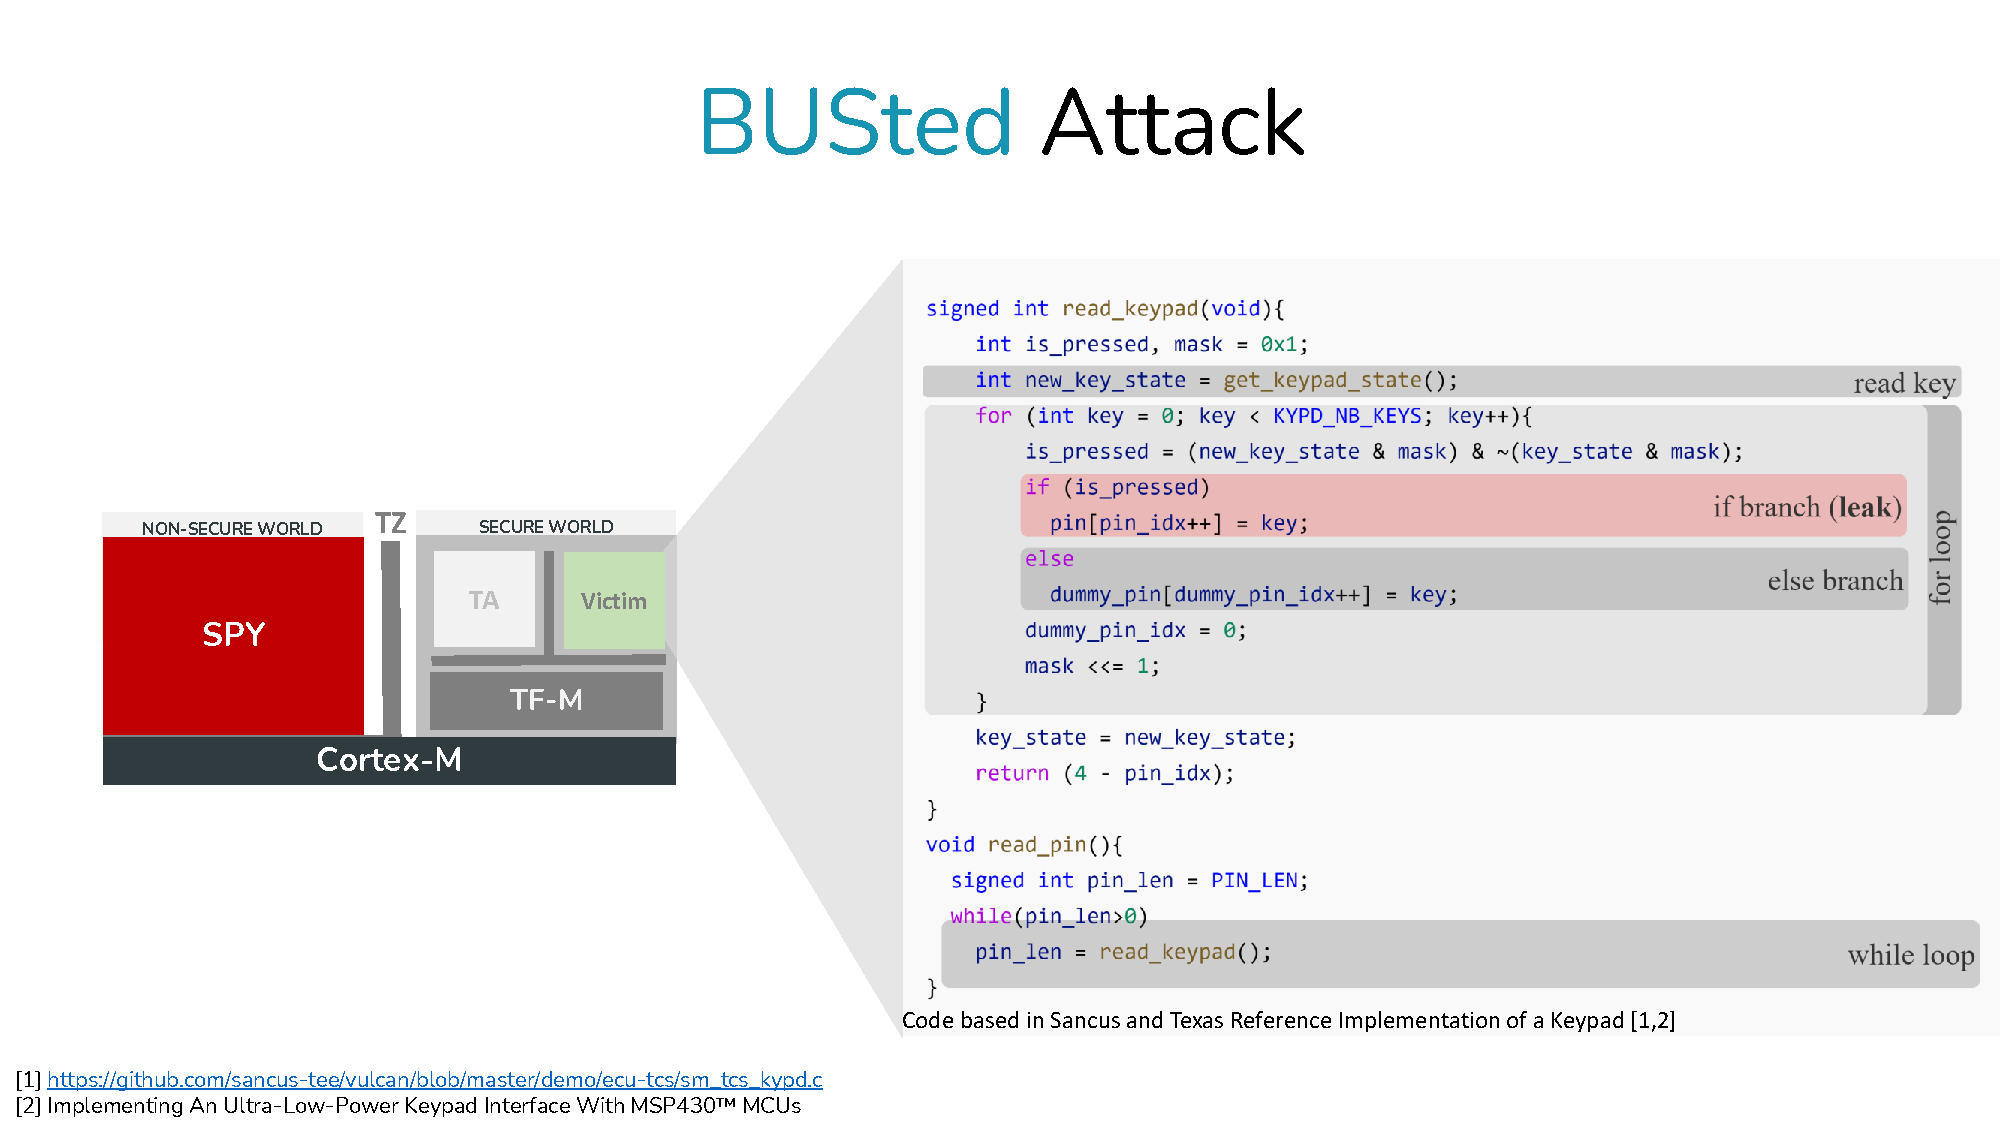
\includegraphics[width=1\textwidth]{img/busted3.pdf}
    \end{center}
\end{figure} 
\end{frame}

\begin{frame}[allowframebreaks]{References}
\tiny
\printbibliography
\end{frame}
\end{document}
